\documentclass[conference]{IEEEtran}

\usepackage{cite}
\usepackage{amsmath}
\usepackage{graphicx}

\title{An Improvement of Weighted PageRank to Handle the Zero Link Similarity}
\author{\IEEEauthorblockN{Muhammad Ogin Hasanuddin}\\
\IEEEauthorblockA{\textit{Fakultas Teknologi Informasi}\\
\textit{Institut Teknologi Batam}\\
Batam, Indonesia\\
moginh@iteba.ac.id}}

\begin{document}

% Judul
\maketitle

% Abstrak
\begin{abstract}
    The well-known PageRank algorithm makes use of the   link   structure   to   calculate   a   quality   rank   for   pages.   It   basically   delivers
\end{abstract}

% Keywords
\begin{IEEEkeywords}
    PageRank
\end{IEEEkeywords}

% Pendahuluan
\section{Introduction}
Pendahuluan~\cite{brin1998anatomy, xing2004weighted}

% Related works
\section{Related Works}
\subsection{PageRank Algorithm}
sesuatu

\begin{equation}
    r_j = \Sigma_{i \underset{out}{\rightarrow} j} \frac{r_i}{L_{out}(i)}
\end{equation}

\begin{equation}
    \Sigma r_i = 1
\end{equation}

\section{Proposed Algorithm}


\section{Experiment}


\begin{figure}[htpb]
    \centering
    \def\svgwidth{\columnwidth}
    \scalebox{0.8}{\input{gambar1.pdf_tex}}
    \caption{Experiment System Architecture}
\end{figure}

\begin{figure}[htpb]
    \centering
    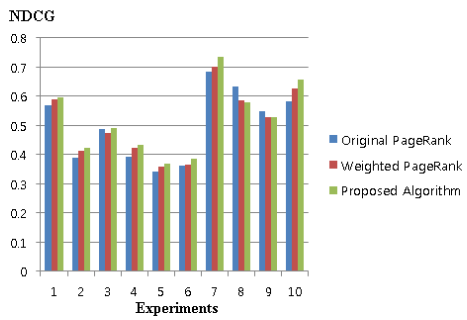
\includegraphics[width=0.4\textwidth]{gambar2.png}
    \caption{Comparison of the original PageRank and the proposed Algorithm }
\end{figure}

\section{Conclusion}

\subsubsection{WeightedPageRank based ion the number of in-links of neighboring pages}


% Referensi
\bibliographystyle{IEEEtran}
\bibliography{references}

\end{document}